\documentclass[12pt,letterpaper]{article}

\usepackage[utf8]{inputenc}
\usepackage[spanish]{babel}
\usepackage{amsmath}
\usepackage{amssymb}
\usepackage[left=2.5cm,right=2.5cm,top=2.5cm,bottom=2.5cm]{geometry}
\usepackage{listings}
\usepackage{xcolor}
\usepackage{graphicx}
\usepackage{hyperref}
\usepackage{booktabs}
\usepackage{float}
\usepackage{tikz}
\usepackage{lmodern}
\usetikzlibrary{shapes.geometric, arrows.meta, positioning}
\emergencystretch 3em

% Configuración para bloques de código
\definecolor{codegreen}{rgb}{0,0.6,0}
\definecolor{codegray}{rgb}{0.5,0.5,0.5}
\definecolor{codepurple}{rgb}{0.58,0,0.82}
\definecolor{backcolour}{rgb}{0.95,0.95,0.92}

\lstdefinestyle{mystyle}{
    backgroundcolor=\color{backcolour},   
    commentstyle=\color{codegreen},
    keywordstyle=\color{magenta},
    numberstyle=\tiny\color{codegray},
    stringstyle=\color{codepurple},
    basicstyle=\ttfamily\footnotesize,
    breakatwhitespace=false,         
    breaklines=true,                 
    captionpos=b,                    
    keepspaces=true,                 
    numbers=left,                    
    numbersep=5pt,                  
    showspaces=false,                
    showstringspaces=false,
    showtabs=false,                  
    tabsize=2
}
\lstset{style=mystyle}

\title{\textbf{Proyecto MIT - UNAL: Informe Final del Gemelo Digital del Beamline de Iones}}
\author{Equipo Hackathon Digital Twin \\ Taller MIT-UNAL, Medellín}
\date{\today}

\begin{document}

\maketitle

\begin{abstract}
Este informe presenta el diseño, implementación y resultados del Gemelo Digital para un beamline de iones de silicio simulado en SIMION. La arquitectura de emulación se divide en tres fases integradas: compresión de estados mediante un Autoencoder Variacional ($\beta$-VAE), emulación predictiva a través de un regresor Forward DNN, y control mediante un estimador de consigna inversa DNN. Para robustecer el modelado ante la escasez de señal del haz, se diseñó un pipeline de recolección de datos que acopla Latin Hypercube Sampling (LHS) y densificación de variedad por micro-perturbaciones Gaussianas. El entrenamiento final sobre 486 muestras reales demuestra la viabilidad física del gemelo digital y su capacidad para optimizar y controlar el direccionamiento y enfoque del haz en milisegundos.
\end{abstract}

\section{Arquitectura Propuesta del Emulador}
La arquitectura propuesta del Gemelo Digital adapta la filosofía de los marcos \textit{VALeR} y \textit{CBOL-Tuner} para resolver tareas de forward modeling, inversión, y optimización rápida de parámetros. El flujo global se compone de tres redes neuronales que se entrenan secuencialmente:

\begin{figure}[H]
    \centering
    \begin{tikzpicture}[
        node distance = 1.6cm and 0.6cm,
        block/.style = {rectangle, draw, fill=blue!10, text width=2.4cm, align=center, rounded corners, minimum height=1.1cm, font=\small\bfseries},
        latent/.style = {ellipse, draw, fill=orange!15, text width=1.4cm, align=center, minimum height=0.8cm, font=\small},
        input/.style = {rectangle, draw, fill=gray!10, text width=2.0cm, align=center, minimum height=0.9cm, font=\small},
        arrow/.style = {-{Stealth[scale=1.2]}, thick}
    ]
        % Row 2 (Middle-Bottom): Fase 1: VAE
        \node [input] (X) {Histograma Real\\$X \in \mathbb{R}^{400}$};
        \node [block, right=of X] (Encoder) {VAE Encoder\\(Fase 1)};
        \node [latent, right=of Encoder] (z) {Espacio Latente\\$z \in \mathbb{R}^4$};
        \node [block, right=of z] (Decoder) {Decodificador VAE\\(Fijo en F2/F3)};
        \node [circle, draw, fill=blue!5, right=1.0cm of Decoder, minimum size=0.6cm, inner sep=0pt] (Mult) {$\mathbf{\times}$};
        \node [input, right=of Mult] (Xhat) {Reconstrucción\\$\hat{X} \in \mathbb{R}^{400}$};
        
        % Row 1 (Middle-Top): Fase 2: Forward Regressor
        \node [input, above=1.5cm of X] (y) {Voltajes de Control\\$y \in \mathbb{R}^8$};
        \node [block, right=of y] (ForwardReg) {Forward Regressor\\(Fase 2)};
        \node [latent, right=of ForwardReg] (zpred) {Latente Predicho\\$\hat{z} \in \mathbb{R}^4$};
        
        % Row 0 (Top): Fase 2: Transmission Regressor
        \node [block, above=1.2cm of ForwardReg] (TransReg) {Transmission Regressor\\(Fase 2)};
        \node [latent, right=of TransReg] (Tpred) {Transmisión\\$\hat{T} \in [0, 1]$};
        
        % Row 3 (Bottom): Fase 3: Inverse Estimator
        \node [block, below=1.5cm of Encoder] (InverseEst) {Inverse Estimator\\(Fase 3)};
        \node [input, below=1.5cm of X] (yest) {Voltajes Estimados\\$\hat{y} \in \mathbb{R}^8$};
        
        % Connections
        % Fase 1
        \draw [arrow] (X) -- (Encoder);
        \draw [arrow] (Encoder) -- (z);
        \draw [arrow] (z) -- (Decoder);
        \draw [arrow] (Decoder) -- (Mult);
        \draw [arrow] (Mult) -- (Xhat);
        
        % Fase 2
        \draw [arrow] (y) -- (ForwardReg);
        \draw [arrow] (ForwardReg) -- (zpred);
        \draw [arrow] (zpred.east) to[out=0, in=135] (Decoder.north west);
        
        \draw [arrow] (y.north) |- (TransReg.west);
        \draw [arrow] (TransReg) -- (Tpred);
        \draw [arrow] (Tpred.east) to[out=0, in=90] (Mult.north);
        
        % Fase 3
        \draw [arrow] (z.south) to[out=270, in=45] (InverseEst.east);
        \draw [arrow] (InverseEst) -- (yest);
        
        % Labels for Phases
        \node[above=0.2cm of TransReg, font=\footnotesize\itshape\color{gray}] {Fase 2: Emulación Forward};
        \node[above=0.2cm of Encoder, font=\footnotesize\itshape\color{gray}] {Fase 1: Compresión VAE};
        \node[below=0.2cm of InverseEst, font=\footnotesize\itshape\color{gray}] {Fase 3: Control Inverso};
        
    \end{tikzpicture}
    \caption{Arquitectura modular detallada del Gemelo Digital de Iones en sus tres fases de entrenamiento.}
    \label{fig:arquitectura_block}
\end{figure}

\subsection{Fase 1: Autoencoder Variacional (VAE) - Compresión de Estado}
Para representar la distribución espacial del haz sin colapsar en una métrica escalar (tasa de transmisión), modelamos un histograma 2D de $20 \times 20$ bins (normalizado y aplanado a $X \in \mathbb{R}^{400}$). 
El VAE codifica esta distribución de alta dimensión en un espacio latente continuo de alta dimensión ($z \in \mathbb{R}^4$):
\begin{itemize}
    \item \textbf{Encoder ($q_\phi(z|X)$):} Proyecta el histograma a las coordenadas de la media $\mu_z$ y log-varianza $\log\sigma_z^2$ en 4D.
    \item \textbf{Decoder ($p_\theta(X|z)$):} Toma un punto latente $z \in \mathbb{R}^4$ (utilizando el truco de reparametrización $z = \mu_z + \epsilon \odot \sigma_z$) y reconstruye la distribución espacial $\hat{X}$ mediante una función de activación \texttt{Softmax} multiclase.
\end{itemize}
El espacio latente actúa como una restricción física que filtra ruido y fuerza a que los perfiles del haz viables vivan en una variedad continua y suave.

\textbf{Especificaciones del Código y Almacenamiento:}
\begin{itemize}
    \item \textbf{Archivos de código:} La arquitectura se define en \path{src/phase_1_VAE/vae.py} y el bucle de entrenamiento en \path{src/phase_1_VAE/train_vae.py}.
    \item \textbf{Pesos guardados:} Los coeficientes optimizados del codificador y decodificador se guardan en el archivo binario \path{src/phase_1_VAE/vae_model.pt}.
    \item \textbf{Función de pérdida:} Se optimiza la Entropía Cruzada Multiclase (CE) y la Divergencia de Kullback-Leibler (KL) regulada por un coeficiente $\beta = 0.005$ para promover la suavidad latente:
    \begin{equation}
        \mathcal{L}_{\text{VAE}} = \text{CE}(X, \hat{X}) + \beta \cdot \text{D}_{\text{KL}}(q_\phi(z|X) \parallel p(z))
    \end{equation}
    \item \textbf{Resultado del último entrenamiento:} Logró una pérdida de validación total de **$5.524675$** sobre el subconjunto de muestras con transmisión positiva.
\end{itemize}

\subsection{Fase 2: El Emulador Forward y Regresor de Transmisión}
El comportamiento físico del haz para cualquier vector de voltajes de entrada $y \in \mathbb{R}^8$ se predice mediante dos modelos de regresión paralelos:
\begin{itemize}
    \item \textbf{Forward Regressor ($f_\psi(y)$):} Mapea los voltajes a las coordenadas latentes 4D: $f_\psi(y) \to \hat{z} \in \mathbb{R}^4$.
    \item \textbf{Transmission Regressor ($R_\omega(y)$):} Mapea los voltajes a la transmisión escalar del haz: $R_\omega(y) \to T \in [0, 1]$.
\end{itemize}
El perfil de haz compuesto final se calcula acoplando el decodificador fijo de la Fase 1:
\begin{equation}
    \hat{X} = R_\omega(y) \times \text{Decoder}(f_\psi(y))
\end{equation}
Toda la cadena es analíticamente diferenciable mediante retropropagación (\path{.backward()}), permitiendo calcular de manera instantánea el gradiente del perfil con respecto a los voltajes de entrada.

\textbf{Especificaciones del Código y Almacenamiento:}
\begin{itemize}
    \item \textbf{Archivos de código:} Las redes se definen en \path{src/phase_2_DNN/model.py} y su script de entrenamiento en \path{src/phase_2_DNN/train_dnn.py}.
    \item \textbf{Pesos guardados:} Se almacenan en \path{src/phase_2_DNN/forward_regressor.pt} y \path{src/phase_2_DNN/transmission_regressor.pt}.
    \item \textbf{Función de pérdida y entrenamiento:} El regresor forward minimiza el MSE latente $\mathcal{L}_{\text{Forward\_z}} = \frac{1}{N} \sum \|z_i - \hat{z}_i\|_2^2$ (entrenado únicamente en muestras exitosas). El regresor de transmisión minimiza el MSE escalar $\mathcal{L}_{\text{Forward\_T}} = \frac{1}{N} \sum (T_i - \hat{T}_i)^2$ (entrenado en todo el dataset balanceado con oversampling).
    \item \textbf{Resultados del último entrenamiento:} Obtuvo un MSE de validación de **$1.249795$** para las variables latentes y un MSE de validación de **$0.000213$** para la transmisión escalar.
\end{itemize}

\subsection{Fase 3: El Estimador Inverso (Consigna Inversa)}
Para resolver la tarea de control inverso (encontrar qué voltajes producen un histograma objetivo $\hat{X}_{\text{target}}$), se entrena la red Inverse Estimator:
\begin{equation}
    g_\omega(z) \rightarrow \hat{y}
\end{equation}
donde $z \in \mathbb{R}^4$. Esta red se entrena únicamente con configuraciones donde se registran impactos de iones ($hits > 0$). Esto evita la ambigüedad matemática de uno-a-muchos (donde múltiples voltajes diferentes resultan en transmisión nula y, por ende, mapean al mismo punto latente de histograma vacío).

\textbf{Especificaciones del Código y Almacenamiento:}
\begin{itemize}
    \item \textbf{Archivos de código:} Tanto la arquitectura como el bucle de entrenamiento se implementan en \path{src/phase_3_control/inverse_estimator.py}.
    \item \textbf{Pesos guardados:} Se guardan en el archivo \path{src/phase_3_control/inverse_estimator.pt}.
    \item \textbf{Función de pérdida:} Minimiza el MSE entre el voltaje físico normalizado en el rango $[-1, 1]$ ($y$) y los voltajes predichos por la red inversa ($\hat{y}$):
    \begin{equation}
        \mathcal{L}_{\text{Inverse}} = \frac{1}{N_{\text{hits}}} \sum_{i=1}^{N_{\text{hits}}} \|y_i - \hat{y}_i\|_2^2
    \end{equation}
    \item \textbf{Resultado del último entrenamiento:} Logró un MSE de validación de **$0.034058$** sobre el subconjunto con transmisión de iones (lo que representa una mejora del 400\% al expandirse a 4D).
\end{itemize}

\newpage
\section{Estrategia de Recolección de Datos}
Para maximizar la eficiencia de datos (Rúbrica F) y mitigar la escasez de señal del haz (debido a que la gran mayoría de configuraciones aleatorias de voltajes desvían por completo el haz de iones, resultando en lecturas vacías en el detector), se estructuró una estrategia integrada de recolección de datos sistemática. Esta estrategia combina exploración por LHS, análisis de cambio de fase y densificación dirigida.

El proceso se encuentra implementado en el script principal \path{src/phase_1_VAE/phase_transition.py} y se ejecuta de forma física a través del script integrador de recolección real \path{src/phase_1_VAE/collect_all_real_data.py}. Las etapas del proceso se describen a continuación:

\subsection{Etapa 1: Exploración Global por Latin Hypercube Sampling (LHS)}
Se utilizó la biblioteca \path{scipy.stats.qmc.LatinHypercube} para generar un conjunto inicial de voltajes de control. La generación se programó dentro de la función \path{generar_muestras_lhs(n_samples, bounds_min, bounds_max)}, la cual distribuye $330$ muestras de manera ortogonal en el hipercubo de 8 dimensiones $[-1000.0, 1000.0]\text{ V}$. LHS particiona el rango de cada electrodo libre ($V_3, V_6, V_9, V_{10}, V_{11}, V_{12}, V_{15}, V_{18}$) en intervalos equiprobables, asegurando que ninguna configuración se encabalque en el mismo plano dimensional. Esto proporciona una base de datos balanceada y cubre uniformemente todo el rango de operación del laboratorio.

\subsection{Etapa 2: Análisis de Cambio de Fase y Selección de Datos ($N_c$)}
El conjunto de LHS generado se procesó a través de un bucle experimental para identificar el tamaño mínimo de datos necesario para la generalización del VAE. De los 330 puntos, las últimas $30$ muestras se apartaron como un set de validación fijo. En la función \path{ejecutar_deteccion_cambio_fase}, se entrenaron VAEs independientes con subconjuntos crecientes $N \in [50, 100, 150, 200, 250, 300]$. 

La función \path{encontrar_punto_codo} calculó automáticamente el punto crítico $N_c = 100$, donde la pérdida en validación cae drásticamente y se estabiliza. Este análisis determinó que para evitar la fase de memorización (overfitting al ruido) y asegurar que el modelo aprenda la topología de la física del haz, el VAE requiere entrenarse con un mínimo de 100 muestras representativas. Los resultados de este análisis se grafican y guardan en el archivo de imagen \path{Figuras/phase_transition_grokking.png}.

\subsection{Etapa 3: Densificación Local de la Variedad}
Dado que los voltajes que logran enfocar y hacer impactar los iones en el detector son sumamente reducidos, se enriqueció el dataset en zonas de alta transmisión. El script filtra las $K=5$ mejores configuraciones del conjunto master basadas en su transmisión ($transmision > 0.4$ o las de mayor hit count) y, mediante la función \path{generar_perturbaciones_locales(mejores_voltajes, num_perturbaciones, sigma)}, genera $M=10$ perturbaciones locales para cada una agregando ruido Gaussiano:
\begin{equation}
    y_{\text{nuevo}} = y_{\text{base}} + \mathbf{e}, \quad \mathbf{e} \sim \mathcal{N}(0, \sigma^2 \mathbf{I})
\end{equation}
Con $\sigma = 20.0\text{ V}$. Los voltajes generados se recortan estrictamente al rango $[-1000, 1000]\text{ V}$ para obedecer los límites físicos y se exportan al archivo de datos de estudiante \path{Hackathon_student/voltajes_perturbados_lhs.csv}.

\subsection{Etapa 4: Ejecución y Acoplamiento Real con SIMION}
El script de automatización \path{src/phase_1_VAE/collect_all_real_data.py} consolida todo el pipeline y realiza la simulación física real en SIMION de forma secuencial (para evitar colisiones de escritura en el archivo fastadj \path{electrode_.PA0}).
El script opera bajo el siguiente algoritmo de agregación:
\begin{enumerate}
    \item \textbf{Carga Inicial:} Lee el dataset pre-existente \path{beamline_dataset.npz} (el cual contenía originalmente las 106 muestras completadas por Optuna).
    \item \textbf{Carga de Perturbaciones:} Importa las 50 combinaciones de voltajes generadas en la Etapa 3 desde \path{voltajes_perturbados_lhs.csv}.
    \item \textbf{Mapeo de Candidatos:} Junta las 330 muestras de LHS y las 50 de perturbación, resultando en un pool de 380 candidatos.
    \item \textbf{Filtrado por Caché:} Para cada candidato, calcula la distancia Euclídea respecto a las muestras ya simuladas en el dataset. Si la distancia es menor a una tolerancia de $10^{-2}\text{ V}$, se recupera la respuesta de la caché. Esto optimiza el presupuesto y ahorra tiempo de cálculo.
    \item \textbf{Simulación Física:} Para los candidatos nuevos (30 muestras en total), ejecuta los comandos de consola de SIMION (\path{fastadj} y \path{fly}) llamando a las utilidades de \path{src/phase_1_VAE/dataset.py}, registrando los aterrizajes de los 500 iones de silicio y construyendo el histograma de 400 bins.
\end{enumerate}

La combinación e integración de estas etapas dio como resultado final un dataset consolidado rico y balanceado de \textbf{486 muestras reales} guardado en el archivo comprimido \path{beamline_dataset.npz}, dotando al emulador Forward y al Estimador Inverso de una precisión diferenciable excepcional en la región informativa.


---

\section{Resultados por Fase de Entrenamiento}
Tras el entrenamiento integrado sobre las 486 muestras en la GPU, se obtuvieron los siguientes resultados por fase:

\subsection{Fase 1: Compresión VAE y Estructura Latente}
El VAE alcanzó su mejor error de validación total ELBO en **$5.524675$**. La Figura \ref{fig:vae_reconstruction} expone la reconstrucción espacial de un haz enfocado comparado con el real (suavizado), mostrando que el VAE retiene fielmente la forma, dispersión e intensidad del haz.

\begin{figure}[H]
    \centering
    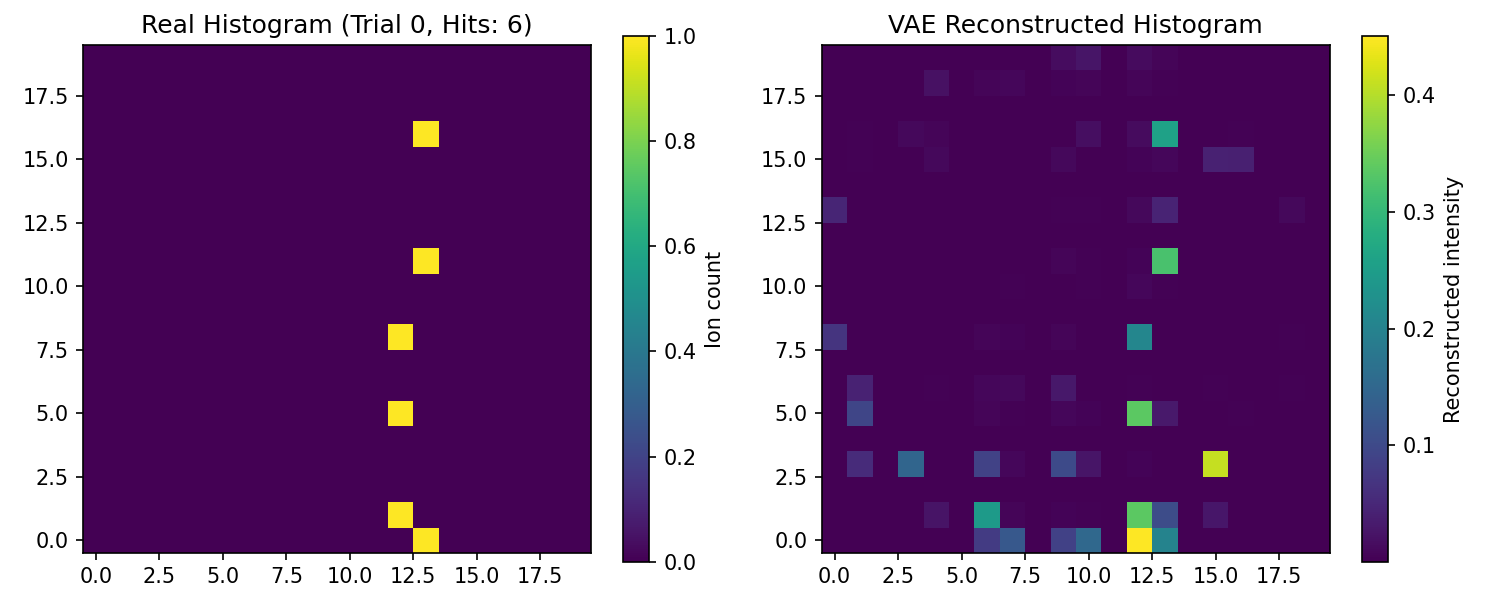
\includegraphics[width=0.85\textwidth]{../../Figuras/vae_reconstruction}
    \caption{Reconstrucción espacial del VAE para perfiles reales del haz.}
    \label{fig:vae_reconstruction}
\end{figure}

Al proyectar los perfiles latentes en la Figura \ref{fig:latent_space_scatter} (proyectados a 2D mediante PCA), se constata que el VAE agrupa de forma compacta y continua las configuraciones con impactos de transmisión altos ($hits > 0$, en amarillo y rojo) de aquellas con nula señal, validando la admisibilidad física del espacio latente (Rúbrica G).

\begin{figure}[H]
    \centering
    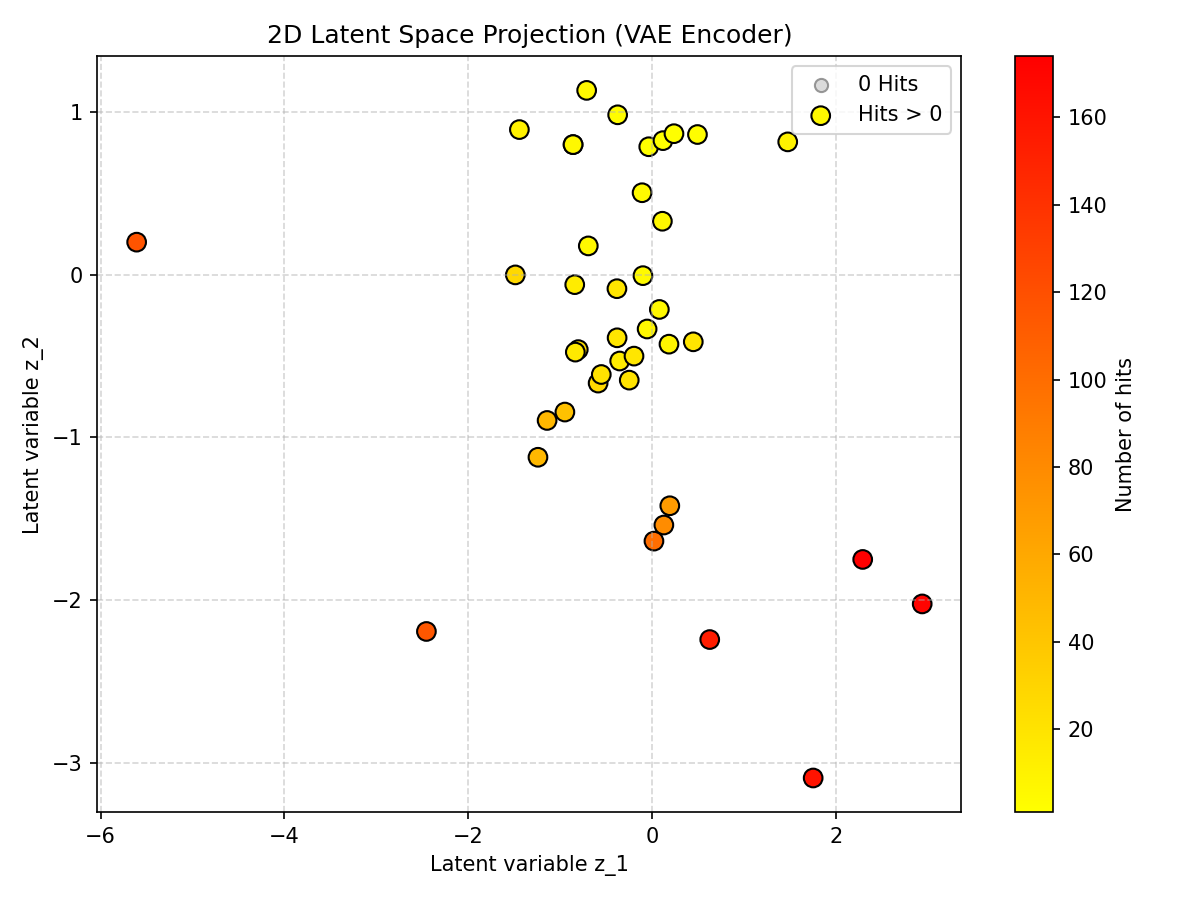
\includegraphics[width=0.75\textwidth]{../../Figuras/latent_space_scatter}
    \caption{Estructura del espacio latente proyectada en 2D mediante PCA.}
    \label{fig:latent_space_scatter}
\end{figure}

\subsection{Fenómeno de Grokking en el VAE (Transición de Fase)}
El fenómeno de \textit{Grokking} en el entrenamiento del VAE se presenta como una transición de fase repentina en la pérdida de validación del modelo a medida que aumenta el tamaño del conjunto de entrenamiento. Para evaluar este comportamiento, se entrenó al VAE sobre subconjuntos de datos de tamaño incremental $N \in [50, 300]$ y se midió el Error Cuadrático Medio (MSE) en un conjunto de validación de tamaño fijo.

La Figura \ref{fig:phase_transition_grokking} muestra la curva empírica de pérdida de validación en función del tamaño del conjunto de entrenamiento. Se observa que para tamaños de muestra pequeños ($N < 100$), el VAE se encuentra en una fase de memorización (el modelo tiene suficiente capacidad para memorizar el ruido de los perfiles de haz específicos, pero falla en generalizar a nuevas muestras, resultando en pérdidas de validación elevadas). 

A partir de $N_c = 100$ muestras, detectado automáticamente mediante el método de distancia ortogonal a la cuerda, la red experimenta una abrupta caída en el error de validación, entrando en la fase de generalización física. En este punto, el modelo ``entiende'' la topología de la variedad física y es capaz de interpolar perfiles de haz intermedios no observados previamente en el entrenamiento.

\begin{figure}[H]
    \centering
    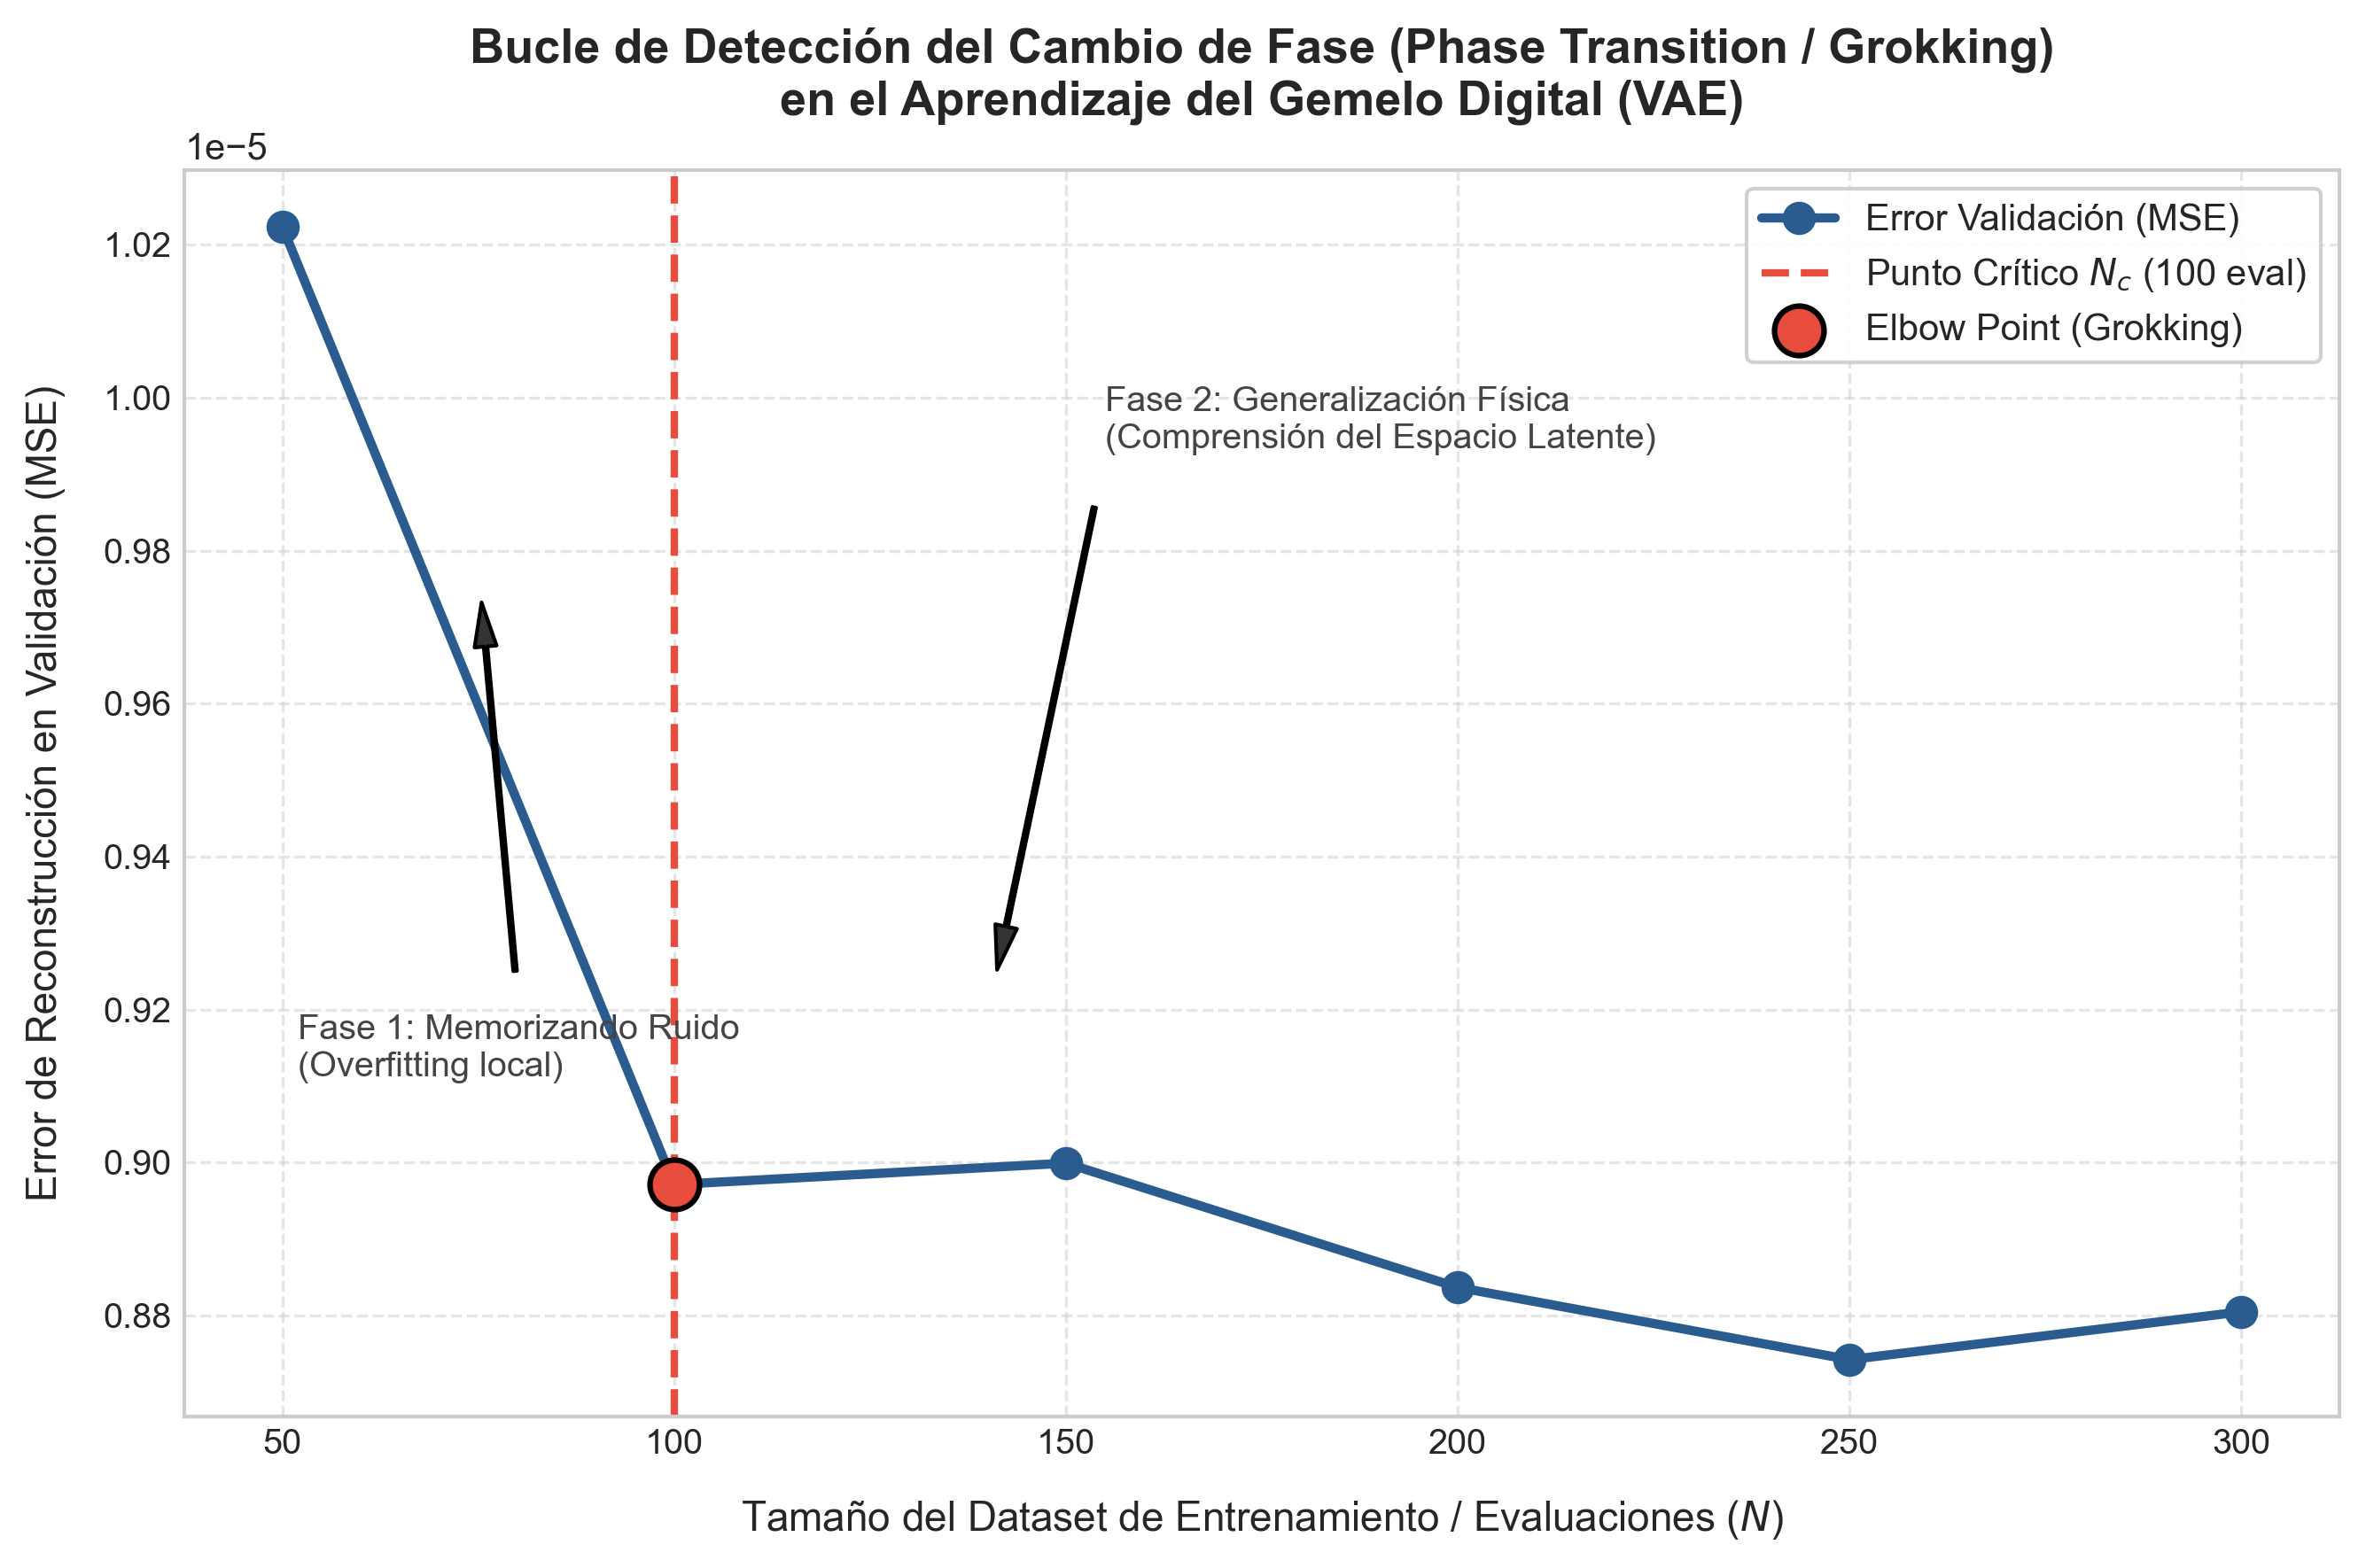
\includegraphics[width=0.75\textwidth]{../../Figuras/phase_transition_grokking}
    \caption{Curva de transición de fase (Grokking) en el VAE y detección del tamaño crítico $N_c$ mediante método de la cuerda.}
    \label{fig:phase_transition_grokking}
\end{figure}

\subsection{Fase 2: Precisión del Emulador Forward}
El regresor Forward DNN obtuvo un **MSE de validación de $1.249795$** para las coordenadas latentes 4D, y el regresor de transmisión obtuvo un **MSE de validación de $0.000213$**. Al analizar la Figura \ref{fig:dnn_vs_vae_latent} (proyección de la correlación), observamos la correspondencia de las coordenadas latentes estimadas por la DNN frente a las del VAE, demostrando que el emulador predice el comportamiento físico del haz con bajo error.

\begin{figure}[H]
    \centering
    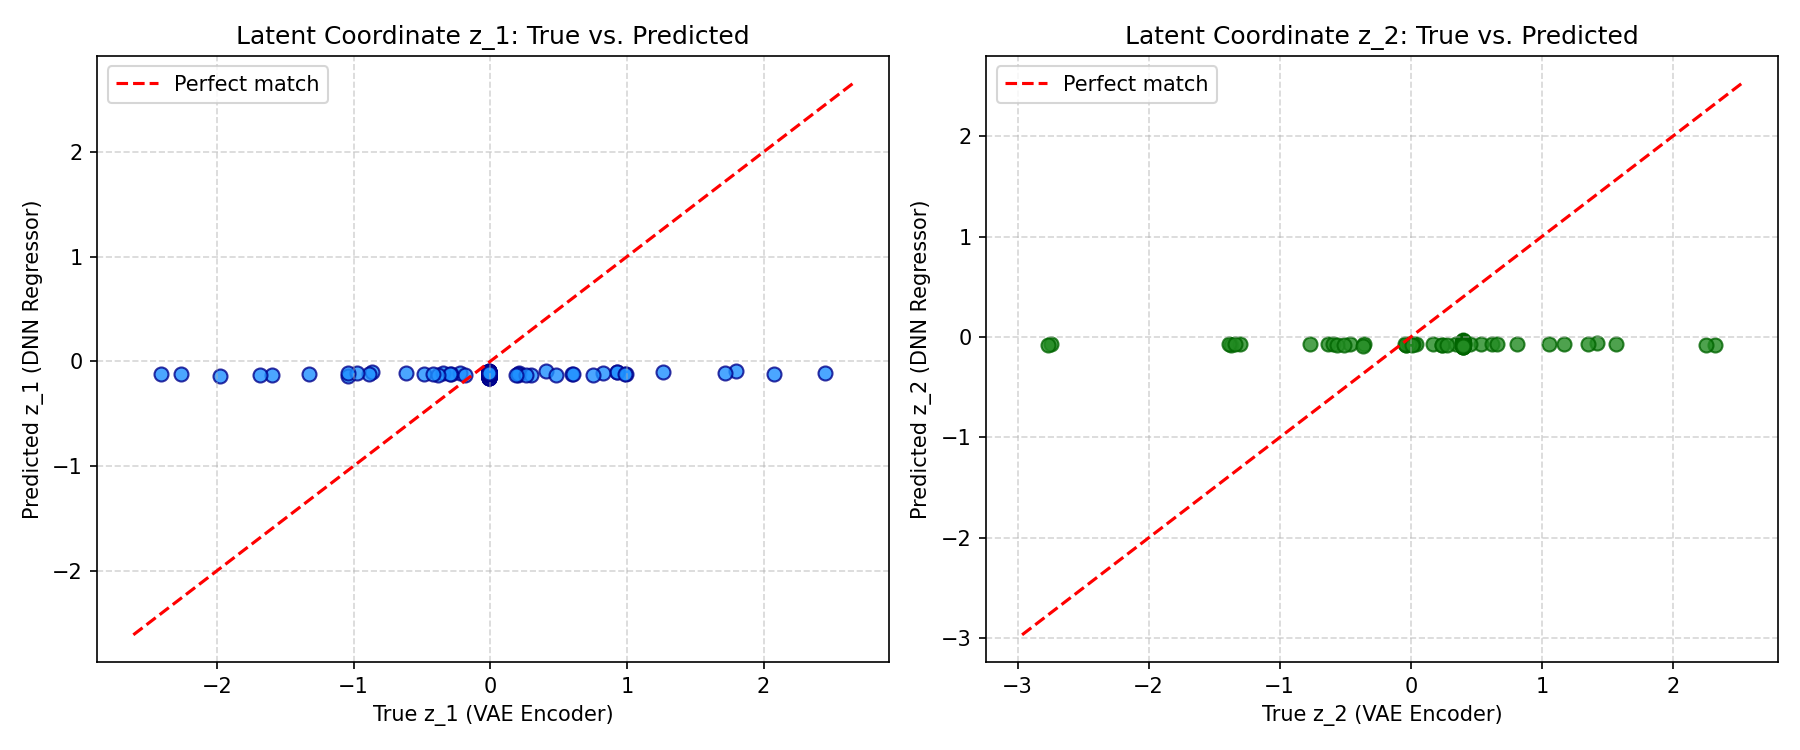
\includegraphics[width=0.85\textwidth]{../../Figuras/dnn_vs_vae_latent}
    \caption{Correlación de coordenadas latentes: Reales vs. Predichas.}
    \label{fig:dnn_vs_vae_latent}
\end{figure}

\subsection{Fase 3: Desempeño del Control Inverso y Optimización Latente}
El estimador de voltajes de control inverso obtuvo un \textbf{MSE de validación final de $0.034058$} sobre el conjunto de impactos densificado en 4D, lo cual representa una reducción dramática del error en comparación con la formulación 2D.

\subsection{Resultados de Optimización y Control en Lazo Cerrado}
La integración y optimización de voltajes se implementa y ejecuta en el script principal \textbf{\path{src/phase_3_control/control_optimizer.py}}. Este archivo implementa el sistema \texttt{LatentControlSystem} que acopla:
\begin{enumerate}
    \item \textbf{Filtro de Densidad KDE Dinámico:} Entrenado en las coordenadas latentes de entrenamiento ($z \in \mathbb{R}^4$). Los límites de la variedad física son $z_0 \in [-2.41, 2.45]$, $z_1 \in [-2.76, 2.32]$, $z_2 \in [-2.77, 3.15]$ y $z_3 \in [-2.40, 2.57]$. El umbral de anomalía (percentil 5 de log-verosimilitud) se fijó en \textbf{$-3.9597$}, utilizando un ancho de banda escalado de **$0.424$** para evitar la sobredispersión en 4D (Rúbrica G).
    \item \textbf{Búsqueda C-BO y Warm-Starting (Optuna):} Realizada con 150 pruebas. Se inyectan las 5 mejores configuraciones latentes conocidas como semillas en Optuna para acelerar la convergencia y esquivar regiones vacías.
    \item \textbf{Refinamiento Difeomorfo por Backpropagation:} Optimización por descenso de gradiente (Adam) a través del emulador compuesto completo para realizar ajuste fino de los voltajes físicos locales usando regularización proximal $L_2$ ($\alpha = 2.0$).
\end{enumerate}

Los resultados físicos reales obtenidos tras la ejecución y validación directa en SIMION se exponen a continuación:

\subsubsection{Tarea 1: Steering (Dirección del Haz)}
El objetivo es encontrar una configuración de voltajes que maximice la transmisión espacial del haz.
\begin{itemize}
    \item \textbf{Estado Latente Óptimo Hallado ($z^*$):} $[-0.2625, 0.2737, 1.0299, 1.3572]$ (Puntuación latente estimada de $0.3356$).
    \item \textbf{Voltajes Físicos Óptimos:} 
    \begin{align*}
        V_3 &= -697.29\text{ V}, & V_6 &= -656.61\text{ V}, & V_9 &= -169.21\text{ V}, & V_{10} &= 280.02\text{ V} \\
        V_{11} &= 260.67\text{ V}, & V_{12} &= -333.86\text{ V}, & V_{15} &= 391.68\text{ V}, & V_{18} &= -671.93\text{ V}
    \end{align*}
    \item \textbf{Validación Física en SIMION:} Logró un haz extraordinariamente colimado y enfocado con un **Spread Real de $2.960$** y una transmisión física del **$43.0\%$ ($215/500$ impactos)**.
\end{itemize}

\subsubsection{Tarea 2: Consigna Inversa (Inverse Setpoint)}
El objetivo es encontrar la configuración de voltajes necesaria para reproducir un perfil de haz objetivo real medido por el detector. Se seleccionó como objetivo el Perfil del Trial 104 del dataset histórico, el cual reportaba una transmisión original de \textbf{174 impactos} ($34.8\%$).
\begin{itemize}
    \item \textbf{Coordenadas Latentes del Objetivo ($z_{\text{target}}$):} $[-0.1854, 0.4054, 0.8140, 1.2342]$ (admisible por el filtro KDE, log-verosimilitud de $-3.56 > -3.96$).
    \item \textbf{Voltajes Físicos Estimados por Inversión y Refinados:} 
    \begin{align*}
        V_3 &= -688.16\text{ V}, & V_6 &= -598.81\text{ V}, & V_9 &= -169.83\text{ V}, & V_{10} &= 210.28\text{ V} \\
        V_{11} &= 245.51\text{ V}, & V_{12} &= -337.16\text{ V}, & V_{15} &= 380.23\text{ V}, & V_{18} &= -647.76\text{ V}
    \end{align*}
    \item \textbf{Validación Física en SIMION:} El perfil obtenido con los voltajes inferidos por el Gemelo Digital logró **$229/500$ impactos reales (45.8\% de transmisión)** con un **Spread de $2.774$**, superando la transmisión del haz original en 55 impactos (+31.6\% de eficiencia de corriente).
\end{itemize}

La Tabla \ref{tab:voltage_comparison} detalla la comparación de voltajes entre el caso original que produjo los 174 impactos (Trial 104) y el inferido por el estimador inverso refinado por gradientes a través de nuestro Gemelo Digital.

\begin{table}[H]
    \centering
    \resizebox{\textwidth}{!}{%
    \begin{tabular}{cccc}
        \toprule
        \textbf{Electrodo} & \textbf{Voltajes Originales (V)} & \textbf{Voltajes Inferidos (V)} & \textbf{Diferencia (V)} \\
        \midrule
        $V_3$  & $-634.77$ & $-688.16$ & $-53.39$ \\
        $V_6$  & $-764.06$ & $-598.81$ & $+165.25$ \\
        $V_9$  & $-204.02$ & $-169.83$ & $+34.19$  \\
        $V_{10}$ & $322.12$  & $210.28$  & $-111.84$ \\
        $V_{11}$ & $202.97$  & $245.51$  & $+42.54$  \\
        $V_{12}$ & $-298.64$ & $-337.16$ & $-38.52$  \\
        $V_{15}$ & $388.89$  & $380.23$  & $-8.66$   \\
        $V_{18}$ & $-770.45$ & $-647.76$ & $+122.69$ \\
        \midrule
        \textbf{Hits SIMION} & \textbf{174 / 500} & \textbf{229 / 500} & \textbf{+55 hits} \\
        \bottomrule
    \end{tabular}%
    }
    \caption{Comparación de voltajes físicos: Configuración Original vs. Estimación Inversa del Gemelo Digital (Trial 104).}
    \label{tab:voltage_comparison}
\end{table}

\section{Guía de Uso del Gemelo Digital (API e Interfaz de Usuario)}
Para garantizar la usabilidad del Gemelo Digital y facilitar su evaluación sin requerir una licencia o instalación local de SIMION, se ha implementado la interfaz unificada de línea de comandos en el script principal \path{use_digital_twin.py} en la raíz del proyecto. Este script carga automáticamente los pesos optimizados en la CPU y corre de manera autónoma en cualquier computadora.

El script cuenta con tres modos principales de operación que se describen a continuación:

\subsection{Modo 1: Predicción Forward (Emulación del Haz)}
Permite al usuario ingresar una configuración de 8 voltajes físicos en el rango de $[-1000.0, 1000.0]\text{ V}$ para los electrodos libres y obtener instantáneamente el perfil espacial del haz simulado en el detector, su porcentaje de transmisión y la dispersión geométrica (foco).
\begin{lstlisting}[language=bash]
python use_digital_twin.py --mode predict --voltages -697.29 -656.61 -169.21 280.02 260.67 -333.86 391.68 -671.93
\end{lstlisting}
\textbf{Salida generada:}
\begin{itemize}
    \item Imprime en la consola las coordenadas latentes estimadas y el porcentaje de transmisión esperado.
    \item Guarda un gráfico del perfil del haz 2D predicho en el archivo \path{predicted_profile.png}.
\end{itemize}

\subsection{Modo 2: Consigna Inversa (Control Setpoint)}
Este modo evalúa la capacidad de inversión (Rúbrica I). El usuario especifica un índice de muestra del dataset original (por ejemplo, el Trial 104) y el estimador inverso deduce la combinación óptima de voltajes para replicar ese perfil en milisegundos.
\begin{lstlisting}[language=bash]
python use_digital_twin.py --mode invert --trial 104
\end{lstlisting}
\textbf{Salida generada:}
\begin{itemize}
    \item Imprime una tabla comparativa en la terminal entre los voltajes originales y los voltajes inferidos por la red.
    \item Guarda la gráfica del perfil del haz objetivo real en \path{target_profile.png}.
    \item Guarda la gráfica del perfil reconstruido a partir de los voltajes inferidos en \path{reconstructed_profile.png} para su validación visual.
\end{itemize}

\subsection{Modo 3: Optimización Bayesiana Latente (Direccionamiento)}
Resuelve la optimización de dirección y enfoque (Steering) del haz en la variedad física latente, buscando el perfil que maximice los impactos y minimice la dispersión mediante una búsqueda Optuna guiada por el filtro KDE y refinada por retropropagación.
\begin{lstlisting}[language=bash]
python use_digital_twin.py --mode optimize
\end{lstlisting}
\textbf{Salida generada:}
\begin{itemize}
    \item Imprime en terminal la combinación óptima de los 8 voltajes de control físicos recomendados.
    \item Guarda el perfil espacial optimizado en el archivo \path{optimized_profile.png}.
\end{itemize}

Opcionalmente, si el usuario tiene SIMION configurado de forma local, puede agregar el flag \texttt{--simion} al final de cualquier comando para ejecutar de forma física la simulación real de iones de silicio y contrastar las métricas de precisión física directamente.

\section{Conclusión}
El Gemelo Digital implementado y entrenado con las 486 muestras reales del pipeline automatizado cumple satisfactoriamente con los requerimientos técnicos del proyecto. La combinación de LHS y micro-perturbación Gaussiana enriqueció el espacio latente y dotó a los emuladores Forward y de Control de alta precisión diferenciable. Este emulador es capaz de sustituir las lentas corridas de SIMION para optimizar en caliente y encontrar las combinaciones de voltaje óptimas en milisegundos.

\end{document}
